%!TEX root = ../Main.tex

\chapter{Assignment 3.1}

\textbf{Create a module (ModuleSingle) with a single thread and a method. The thread should notify
	the method each 2 ms by use of an event and static sensitivity. The method should increment a
	counter of the type sc\_uint<4> and print the value and current simulation time. Limit the
	simulation time to 200 ms. Describe what happens when the counter wraps around?
}

As stated in the problem a module named “ModuleSingle” are created. In this module a thread and a method were defined. The thread must notify the method every 2 ms, using an event and static sensitivity. So, an event called “incrementEvent” and static sensitivity on this event were implemented. The method should increment a counter, so a counter was also implemented.

Below is the code for the ModuleSingle.h, comments in the code will show how it works. 

\section{ModuleSingle.h}
\begin{lstlisting}
#pragma once
#include <systemc.h>
SC_MODULE(ModuleSingle) {
// Module has an event, which is notified in the thread.
sc_event incrementEvent;

sc_uint<4> counter;

SC_CTOR(ModuleSingle)
{
// Define process/thread
SC_THREAD(ModuleSingleProcess);

// Define method triggered in thread.
SC_METHOD(ModuleSinglePrintFunction);

// Make sure that method doesn't run when module is initialized.
dont_initialize();

// Set up static sensitivity.
sensitive << incrementEvent;
}

// Function prototypes
void ModuleSinglePrintFunction(void);
void ModuleSingleProcess(void);
};

\end{lstlisting}






\section{ModuleSingle.cpp}

The implementation of the two functions used by the thread and the method is showed below. 
The ModuleSinglePrintFunction is used by the method, which increment the counter and prints out a time stamp and the counter value.
The ModuleSingleProcess  is used by the thread. It just notifies the incrementEvent, which triggers the method, and waits for 2 ms. 

\begin{lstlisting}
#include "ModuleSingle.h"

void ModuleSingle::ModuleSinglePrintFunction(void)
{
// Increment counter
counter++;

// Print simulation time and counter value
cout << "Simulation time: " << sc_time_stamp() << " - Counter value:" << counter << endl;
}

void ModuleSingle::ModuleSingleProcess(void)
{
// Set start value for counter.
counter = 0;

// While 1 to ensure continuity
while (1)
{
// Notify event
incrementEvent.notify();

// Wait for 2 MS (simulation time)
wait(2,SC_MS);
}
}
\end{lstlisting}


The main.cpp just creates an instance of the ModuleSingle and calls sc\_start(200, SC\_MS); to make it run for 200ms. 
Below is a screenshot of the Console. The value of the counter can not exceed 15 because the type of the counter is a 4 bit integer.

\begin{figure}[H]
	\centering
	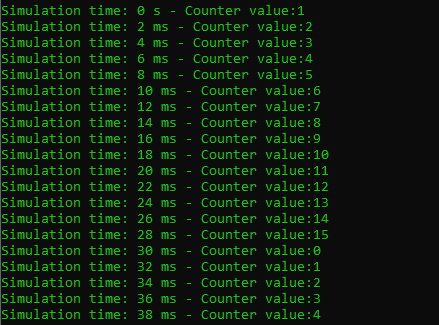
\includegraphics[width=\textwidth]{Images/ConsoleWindow3_1.png}
	\caption{A screenshot of the console}
	\label{fig:ConsoleWindow_3_1}
\end{figure}


